%% 
%% Copyright 2007-2020 Elsevier Ltd
%% 
%% This file is part of the 'Elsarticle Bundle'.
%% ---------------------------------------------
%% 
%% It may be distributed under the conditions of the LaTeX Project Public
%% License, either version 1.2 of this license or (at your option) any
%% later version.  The latest version of this license is in
%%    http://www.latex-project.org/lppl.txt
%% and version 1.2 or later is part of all distributions of LaTeX
%% version 1999/12/01 or later.
%% 
%% The list of all files belonging to the 'Elsarticle Bundle' is
%% given in the file `manifest.txt'.
%% 

%% Template article for Elsevier's document class `elsarticle'
%% with numbered style bibliographic references
%% SP 2008/03/01
%%
%% 
%%
%% $Id: elsarticle-template-num.tex 190 2020-11-23 11:12:32Z rishi $
%%
%%
\documentclass[preprint,12pt]{elsarticle}

%% Use the option review to obtain double line spacing
%% \documentclass[authoryear,preprint,review,12pt]{elsarticle}

%% Use the options 1p,twocolumn; 3p; 3p,twocolumn; 5p; or 5p,twocolumn
%% for a journal layout:
%% \documentclass[final,1p,times]{elsarticle}
%% \documentclass[final,1p,times,twocolumn]{elsarticle}
%% \documentclass[final,3p,times]{elsarticle}
%% \documentclass[final,3p,times,twocolumn]{elsarticle}
%% \documentclass[final,5p,times]{elsarticle}
%% \documentclass[final,5p,times,twocolumn]{elsarticle}

%% For including figures, graphicx.sty has been loaded in
%% elsarticle.cls. If you prefer to use the old commands
%% please give \usepackage{epsfig}

%% The amssymb package provides various useful mathematical symbols
\usepackage{amssymb}
%% The amsthm package provides extended theorem environments
\usepackage{amsmath}

%% The lineno packages adds line numbers. Start line numbering with
%% \begin{linenumbers}, end it with \end{linenumbers}. Or switch it on
%% for the whole article with \linenumbers.
\usepackage{lineno}
\linenumbers

% Load custom packages
\usepackage[
    locale=US,
    separate-uncertainty=true,
    per-mode=fraction,    
    print-unity-mantissa = false
]{siunitx}
\sisetup{math-micro=\text{µ},text-micro=µ}
\usepackage{xcolor}
\usepackage{subcaption}
\usepackage{hyperref}

\usepackage{float}
\usepackage{scrhack}
\floatplacement{figure}{htbp}
\floatplacement{table}{htbp}

\usepackage{multirow}

% schöne Tabellen
\usepackage{booktabs}
\usepackage{multirow}

\journal{Astroparticle Physics}

\begin{document}

\begin{frontmatter}

%% Title, authors and addresses

%% use the tnoteref command within \title for footnotes;
%% use the tnotetext command for theassociated footnote;
%% use the fnref command within \author or \address for footnotes;
%% use the fntext command for theassociated footnote;
%% use the corref command within \author for corresponding author footnotes;
%% use the cortext command for theassociated footnote;
%% use the ead command for the email address,
%% and the form \ead[url] for the home page:
%% \title{Title\tnoteref{label1}}
%% \tnotetext[label1]{}
%% \author{Name\corref{cor1}\fnref{label2}}
%% \ead{email address}
%% \ead[url]{home page}
%% \fntext[label2]{}
%% \cortext[cor1]{}
%% \affiliation{organization={},
%%             addressline={},
%%             city={},
%%             postcode={},
%%             state={},
%%             country={}}
%% \fntext[label3]{}

\title{Simulate muon deflection with PROPOSAL}

%% use optional labels to link authors explicitly to addresses:
%% \author[label1,label2]{}
%% \affiliation[label1]{organization={},
%%             addressline={},
%%             city={},
%%             postcode={},
%%             state={},
%%             country={}}
%%
%% \affiliation[label2]{organization={},
%%             addressline={},
%%             city={},
%%             postcode={},
%%             state={},
%%             country={}}

\author{Pascal Gutjahr}

\affiliation{organization={Dept. of Physics, TU Dortmund University},%Department and Organization
            addressline={August-Schmidt-Straße 1}, 
            city={Dortmund},
            postcode={44227}, 
            state={NRW},
            country={Germany}}

\begin{abstract}
For uncertainty estimation of reconstruction of the muon direction, the 
deflection of muons along a propagated path in ice and water is simulated using 
the tool PROPOSAL (Propagator with optimal precision and optimized speed for all leptons), which considers multiple scattering and stochastic deflection. 
The deflection per interaction spans several 
orders of magnitude with $\theta \in [\SI{e-9}{\degree},\, \SI{1}{\degree}]$ 
for energies $E < \SI{1}{\peta\electronvolt}$ 
and is rather negligible. The accumulated 
deflection of a muon with an energy $E_{\mathrm{\mu}} = \SI{500}{\giga\electronvolt}$ 
after a propagated track is about $\theta_{\text{acc}} = 0.10_{-0.02}^{+0.27}\,\si{\degree}$ 
\alexander{Wie hängt das von der propagierten Distanz ab?}
with a $\SI{95}{\percent}$ central interval, which is in the order of magnitude of 
the directional resolution of 
present neutrino detectors. This deflection can be simply parametrized in 
dependence of the final muon energy. Furthermore, the deflections are compared to the results 
of the propagation tools MUSIC and GEANT4 and all deflections are in good 
agreement. 

\end{abstract}

%%Graphical abstract
\begin{graphicalabstract}
%\includegraphics{grabs}
\end{graphicalabstract}

%%Research highlights
\begin{highlights}
\item Stochastic muon deflection implemented into PROPOSAL
\item Comparison of deflections of MUISIC, GEANT4 and PROPOSAL
\item Third degree polynomial fit of muon deflection 
\item Theoretical estimation of angular uncertainty on directional muon reconstruction 
\item (NN-based parametrization of muon deflection distribution? --> useful?!) 
\end{highlights}

\begin{keyword}
%% keywords here, in the form: keyword \sep keyword

%% PACS codes here, in the form: \PACS code \sep code

%% MSC codes here, in the form: \MSC code \sep code
%% or \MSC[2008] code \sep code (2000 is the default)

Neutrino Astronomy \sep Point-Source-Analysis \sep Angular \sep Resolution \sep Machine Learning \sep (!maximum of 6 keywords!)

\end{keyword}

\end{frontmatter}

%% \linenumbers

%% main text
 
\section{Introduction}\label{sec:introduction}
Neutrinos can cross the universe all the way to earth, since they are 
nearly massless and not charged. On earth, neutrinos can interact 
with a nucleus and produce an electron, muon or tau in the charged current 
via the weak interaction \cite{}. These charged daughter particles are very 
high-energetic and emit Cherenkov light \cite{}, which can be detected 
by large neutrino telescopes like IceCube \cite{IceCube_Instrumentation} or 
KM3NeT \cite{KM3NeT_Design}. 
By the reconstruction of the direction of the daughter particles, the direction 
of the original neutrino can be inferred. The angular resolution is at its 
best for muons, since they can travel up to a few kilo meters due to their 
large mass, instead of the much lighter electron and tau - which decays almost 
instantly. Current angular resolutions are 
$\Phi_{\text{I}} > \SI{0.1}{\degree} - \SI{0.3}{\degree}$ for energies 
$E \in [\SI{3}{\tera\electronvolt},\,\SI{3}{\peta\electronvolt}]$ in IceCube 
\cite{IceCube_Resolution2021} 
and 
$\Phi_{\text{K}} < \SI{0.2}{\degree}$ for $E > \SI{10}{\tera\electronvolt}$ in 
KM3NeT/ARCA \cite{KM3NeT_Resolution2021}.
Since muons do up to $10,000$ interactions along their propagation while they 
are deflected in each interaction, it is important to study if the accumulated 
deflection along a track impacts the angular resolution of current 
neutrino detectors. 

For this purpose, the lepton propagation 
tool PROPOSAL \cite{koehne2013proposal, dunsch_2018_proposal_improvements} is used to study the muon deflection per interaction in 
Section~\ref{sec:defl_per_int} and the 
accumulated deflection in Section~\ref{sec:accum_defl}. Furthermore, 
the distribution of deflections for given energies and propagation distances 
is parametrized using a neural network in Section~\ref{sec:nn_defl}. The 
paper concludes with a summarized overview in Section~\ref{sec:conclusion}.


% Überlick: 
% Neutrinos kommen aus dem Universum -> fliegen auf Erde -> WW mit Kern 
% -> e,mu,tau entstehen -> geladene hochenergetische Teilchen -> Cherenkov Licht 
% -> kann mit Neutrinodetektoren (wie IceCube und KM3NeT) gemessen werden 
% -> Richtungsrekonstruktion ->
% Rückschluss auf Richtung, aus der das Neutrino entsendet wurde

% -> Myonen haben die beste Richtungsauflösung (Auflösung von IceCube und KM3NeT), 
% da sie aufgrund ihrer hohen Masse 
% eine deutlich größere Strecke zurücklegen können, als elektronen und taus, welche 
% sofort zerfallen -> da myonen entlang ihrer propagierten strecke bis zu 10.000 
% wechselwirkungen durchführen können und sie in jeder einzelnen abgelenkt wird, 
% gilt es nun zu überprüfen, ob die ablenkung der myonen die Richtungsauflösung 
% beeinflusst.

% To determine 
% the position of extraterrestrial neutrino sources more precisely, neutrino 
% experiments are constantly being optimized.

% Neutrinos have a major role to play in the study of the universe. 
% The direction of the original 
% neutrino - emitted by extraterrestrial sources - can be inferred by 
% reconstructing the direction of the daughter 
% particles, which are produced in charged currents.



\section{Overview of the Simulation Tool PROPOSAL}\label{sec:proposal}
The tool PROPOSAL propagates charged leptons and photons through media und is 
used in this paper to simulate the deflection of muons. For this purpose, 
negative charged muons $\mu^-$ are propagated through the media ice and water 
to estimate the deflection for IceCube and KM3NeT/ARCA. All relevant muon interaction types 
as bremsstrahlung \cite{KKP_1995, Karnaukhov_1999}, photonuclear interaction \cite{Abramowicz_1997} with 
shadowing \cite{ButkevichMikheyev_2002}, electron pair production \cite{KKP_proc} with corrections for the 
interaction with atomic electrons \cite{Kelner_1998}, 
ionization by Bethe-Block formula with corrections for muons \cite{Rossi} and decay are provided. The interaction processes are sampled by their cross section. Since bremsstrahlung interactions can be 
arbitrary small due to a massless exchange particle, the photon, an energy cut is introduced to avoid an infinite number of bremsstrahlung interactions 
and furthermore to speed up the propagation process. 
The limit is applied with a minimum energy loss
\begin{equation}
    E_{\text{loss,min}} = \min{(E \cdot \texttt{v\_cut}, \texttt{e\_cut})}\,,
\end{equation}
using two parameters - a relative and total energy cut denoted as 
$\texttt{v\_cut}$ and $\texttt{e\_cut}$ with particle energy $E$. The uncertainties are small 
for a relative energy cut $\texttt{v\_cut}\ll 1$, which increases the 
CPU runtime.
A sampled energy loss 
$E_{\text{loss}} < E_{\text{loss,\,min}}$ builds an integrated part of a 
stochastic energy loss referred to as continuous energy loss. The 
propagation process is defined by an initial energy $E_{\text{i}}$ and 
two stopping criteria - a final energy $E_{\text{f,\,min}}$ and a 
maximum propagation distance $d_{\text{min}}$. If the last interaction of 
a propagation is sampled by a stochastic interaction, the true final energy 
$E_{\text{f}}$ can become lower and the 
propagation distance $d$ can be higher than the required limits. 
The deflections for stochastic interactions are parametrized by Van Ginneken 
in \cite{Van_Ginneken} with a direct calculation of the deflection in 
ionization using four-momentum conservation. 
Furthermore, there are parametrizations for deflections given in GEANT4 \cite{GEANT4} 
for bremsstrahlung and photonuclear interaction, which 
are available in PROPOSAL, too.
To estimate the deflection along 
a continuous energy loss, multiple scattering established by Moliére 
\cite{moliere_scattering} and the gaussian approximation by Highland 
can be chosen \cite{HIGHLAND_1975}. 
The deflection angle in the plane perpendicular to the muon direction is 
sampled uniformly between $0$ and $2\pi$.
The latest updates with a detailed description of the whole tool can be found 
in \cite{phd_soedingrekso}.
All simulations are done with PROPOSAL $7.3.0$.

\section{Muon deflection per Interaction}\label{sec:defl_per_int}
First, the stochastic deflections introduced by \cite{Van_Ginneken} implemented 
in PROPOSAL are investigated in relation to the two multiple scattering methods. Thereby, the deflections per interaction are presented 
for each interaction type and the total amount in Figure~\ref{fig:defl_per_int}. A single deflection 
extend over several orders of magnitude with a median of $\SI{1.5e-6}{\degree}$
and a $\SI{95}{\percent}$ central interval of $[\SI{1.6e-7}{degree}, \,\SI{2.8e-4}{degree}]$. \textcolor{red}{achtung, ohne cont! - muss noch geändert werden}
It thus follows that the deflections are primarily dominated by multiple scattering, except for a few outliers. 

\begin{figure}
    \centering 
    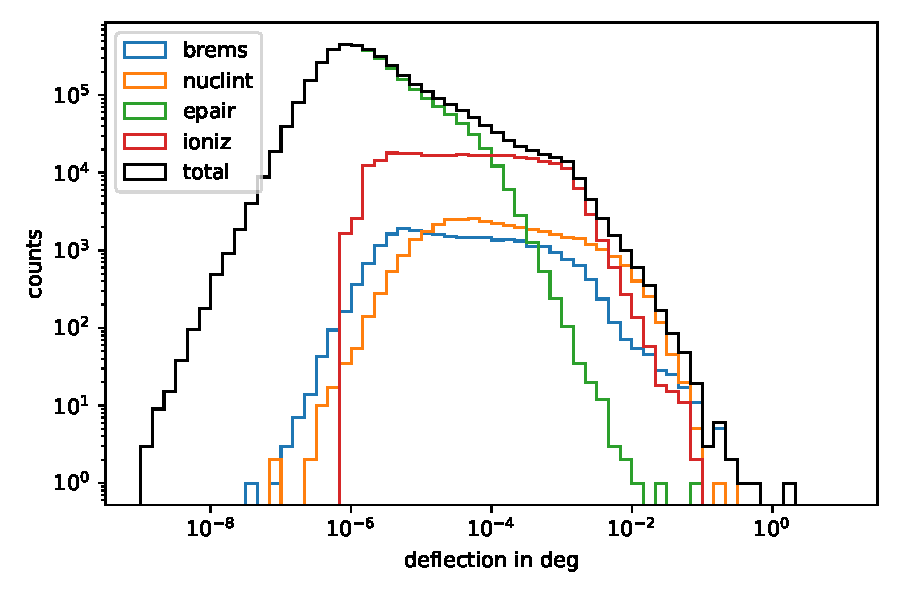
\includegraphics[width=0.8\textwidth]{figures/1PeV_1TeV_1000events.pdf}
    \caption{The propagation is done for $\num{1000}$ 
    muons from $E_{\text{i}} = \SI{1}{\peta\electronvolt}$ to $E_{\text{f,\,min}} = \SI{1}{\tera\electronvolt}$ using $\texttt{e\_cut} = \SI{500}{\mega\electronvolt}$ and $\texttt{v\_cut} = 0.05$ in ice. Two simulations 
    are done to check both multiple scattering methods Molière and Highland. The total distribution is done for all stochastic processes and Molière. Details are presented in 
    Table~\ref{tab:defl_per_int}.}
    \label{fig:defl_per_int}
\end{figure}

\begin{table}
    \centering 
    \caption{The medians of deflections per interaction from Figure~\ref{fig:defl_per_int} are presented for each interaction type and the total distribution with the upper and lower limits of the $\SI{95}{\percent}$ 
    central content levels.}
    \begin{tabular}{ccccc}
        \toprule 
        brems & nuclint & epair & ioniz & total \\
        $\theta\,/\,\SI{e-5}{\degree}$ & $\theta\,/\,\SI{e-4}{\degree}$ & $\theta\,/\,\SI{e-6}{\degree}$ & $\theta\,/\,\SI{e-5}{\degree}$ & $\theta\,/\,\SI{e-6}{\degree}$\\
        \midrule 
        $3.8_{-0.1}^{+297}$ & $1.2_{-0.4}^{+96}$ & $1.3_{-0.2}^{+42}$ & $4.4_{-0.1}^{+181}$& $1.5_{-0.2}^{+279}$\\ 
        \bottomrule
    \end{tabular}
    \label{tab:defl_per_int}
\end{table}
\textcolor{red}{füge moliere und highland sowohl im plot, als auch in der tabelle hinzu. überprüfe dann nochmal die werte! ändere die werte von total auf die neue total kurve mit multiple scattering (moliere)}
\section{Accumulated Muon Deflection}\label{sec:accum_defl}

As shown in Section~\ref{sec:defl_per_int}, in general the deflection per interaction 
is lower $\sim\SI{1}{\degree}$. Since these deflections accumulate along the 
propagation path, the angle between the incoming muon direction and the outgoing 
muon direction is analyzed. The deflection results as a limit on the 
angular reconstruction accuracy.

At first, the deflections in PROPOSAL are compared to 
the tools MUSIC \cite{MUSIC,comparison_MUSIC_GEANT4_2009} and GEANT4 \cite{GEANT4}.
MUSIC (MUon SImulation Code) is a tool to simulate the propagation of muons 
through media like rock and water considering the same energy losses as in 
PROPOSAL. Also, the losses are divided into continuous and stochastic 
energy losses by a relative energy cut. Several cross-sections, multiple scattering 
methods and parametrizations for stochastic deflection are 
available. For these studies, it is chosen bremsstrahlung \cite{Bremsstrahlung_KKP}, 
nuclear interaction \cite{nulcint_bugaev_Shlepin, bugaev_1980_defl,bugaev_1981_defl} 
and electron pair production \cite{epair_kelner,epair_kokoulin_petrukhin}, 
which deflections are parametrized by \cite{Van_Ginneken}. 
Also, ionization is treated as a stochastic process with the Bethe-Bloch 
formula including knock-on electron production. As scattering, the gaussian 
approximation \cite{HIGHLAND_1975} is set. 
GEANT4 is another common toolkit to simulate the passage of particles through 
a medium with several possibilities and a focus on high-energy 
particle accelerators \cite{GEANT4}. 

A comparison of all three tools is done in Figure~\ref{fig:compare_MUSIC} 
with four different settings in PROPOSAL for the 
accumulated deflection angle $\theta_{\text{acc}}$ and the lateral displacement
$x$. The deflection angles are very similar in all cases. The 
displacement is dominated by GEANT4 and PROPOSAL with Molière scattering, which 
leads to the largest deflections and thus to a larger displacement. 
PROPOSAL with Highland scattering and MUSIC have less outliers, since large 
deflections are neglected in the Gaussian approximation \cite{HIGHLAND_1975}. 
The combination of Highland and \cite{Van_Ginneken} leads to the smallest 
displacement, since in nuclear interaction, the sampling from the root mean squared angle in the 
exponential distribution neglects outliers to larger angles.

Detailed information are given in Table~\ref{tab:compare_MUSIC}. In GEANT4, the 
largest deflections result with $\overline{\theta} = \SI{0.27}{\degree}$ 
and $\overline{x} = \SI{3.3}{\meter}$. The lowest values $\overline{\theta} = \SI{0.22}{\degree}$ and 
$\overline{x} = \SI{2.6}{\meter}$ result in MUSIC. The results of PROPOSAL lay between 
these two tools for all four settings which approves the 
correctness of PROPOSAL.

A measurement of muon deflection in low-Z materials was done in \cite{attwood_2006}. 
From this it can be seen that for $Z < 4$ the scattering angle is overestimated 
by Molière scattering in GEANT4. Hence, the lower scattering in PROPOSAL leads 
to a better precision especially in the region of outliers. The simulation is 
done in liquid $\text{H}_2$ with a thickness of $\SI{109}{\milli\meter}$ and an 
initial particle energy of $E_{\mathrm{i}} = \SI{199}{\mega\electronvolt}$. 
The result is presented in Figure~\ref{fig:attwood_comparison}.
\begin{figure}
    \centering 
    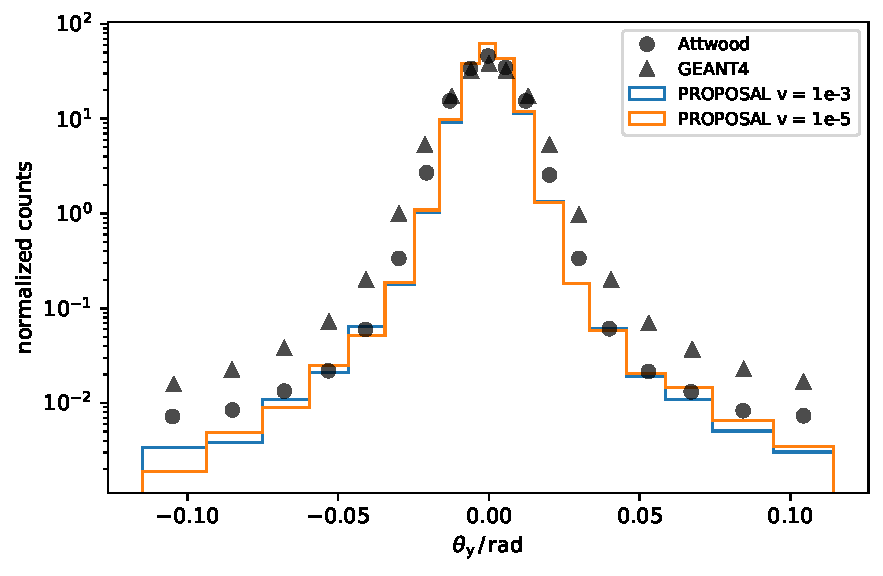
\includegraphics[width=0.8\textwidth]{../../deflection/plots/FINAL/attwood_comparison_moliere_E199MeV_final.pdf}
    \caption{In total $\num{e5}$ muons with $E_{\mathrm{i}} = \SI{199}{\mega\electronvolt}$ are propagated through 
    $\SI{109}{\milli\meter}$ of liquid $\text{H}_2$. In PROPOSAL, the simulation is done 
    for two different energy cuts $\texttt{v\_cut} = \num{e-3}$ and $\texttt{v\_cut} = \num{e-5}$ using Molière scattering.
    Measured data of Attwood and simulation data of GEANT4 are taken from \cite{attwood_2006}. The figure presents 
    the normalized counts in dependence of the projected scattering angle $\theta_{\mathrm{y}}$ in radians. At small deflections, PROPOSAL 
    is underestimating, but at larger deflections the result seems to be more accurate than GEANT4's.}
    \label{fig:attwood_comparison}
\end{figure}

% \begin{itemize}
%     \item this is MUSIC: 
%     \item electron pair production:  Kelner-..[\cite{epair_kelner,epair_kokoulin_petrukhin}], deflection [\cite{Van_Ginneken}]
%     \item bremsstrahlung: Kelner, Kokoulin andPetrukhin
%     [\cite{Bremsstrahlung_KKP}], deflection [\cite{Van_Ginneken}] 
%     \item inelastic scattering: shlepin and Bugaev [\cite{nulcint_bugaev_Shlepin}], \cite{bugaev_1980_defl,bugaev_1981_defl} (überprüfe, ob genau diese referenz auch im GEANT4 verwendet wird!!!)
%     \item ionization: treated as stochastic process (Bethe-Bloch formula) including knock-on electron production, but no deflection
%     \item scattering: gaussian approx \cite{HIGHLAND_1975}
% \end{itemize}


\textcolor{red}{was macht GEANT4 mit ioniz?}
% \textcolor{red}{Moliere beschreibt nur die Winkeländerung, jedoch nicht die laterale Verschiebung. Wie machen wir das mit der 
% laterale Verschiebung in PROPOSAL für Moliere? Gaussian approx berücsichtigt die Verschiebung}

% \begin{itemize}
%     \item this is GEANT4
%     \item electron pair production: 
%     \item bremsstrahlung:
%     \item inelastic scattering: cross-section \cite{Borog:1975_inelastic}, deflection \cite{Borog:1977_inelastic,Borog:1975_inelastic}
%     \item ionization:
%     \item scattering:
% \end{itemize}

% \begin{itemize}
%     \item this is PROPOSAL
%     \item electron pair production: KelnerKokoulinPetrukhin (Proc. 12th ICCR (1971), 2436) with corrections for the interaction with atomic electrons (Phys. Atom. Nucl. 61 (1998), 448) [\cite{}], deflection \cite{Van_Ginneken}
%     \item bremsstrahlung: KelnerKokoulinPetrukhin (Preprint MEPhI (1995) no. 024-95) and (Phys. Atom. Nucl. 62 (1999), 272) [\cite{}], deflection \cite{Van_Ginneken,GEANT4}
%     \item inelastic scattering: AbramowiczLevinLevyMaor97 (arXiv::hep-ph/9712415) \cite{} with shadowing ButkevichMikheyev (JETP 95 (2002), 11) \cite{}, deflection \cite{Van_Ginneken, Borog:1977_inelastic,Borog:1975_inelastic}
%     \item ionization: BetheBlochRossi Ionization described by Bethe-Bloch formula with corrections for muons and taus by (B. B. Rossi. Prentice-Hall, Inc., Englewood Cliffs, NJ, 1952) [\cite{}], deflection [direct calculation using four-momentum transfers]
%     \item scattering: \cite{HIGHLAND_1975,moliere_scattering}
% \end{itemize}


\begin{figure}
    \centering
    \subcaptionbox{
        The accumulated deflection $\theta_{\mathrm{acc}}$ in degree is very similar in all cases.
        \label{fig:compare_MUSIC_degree}}
        {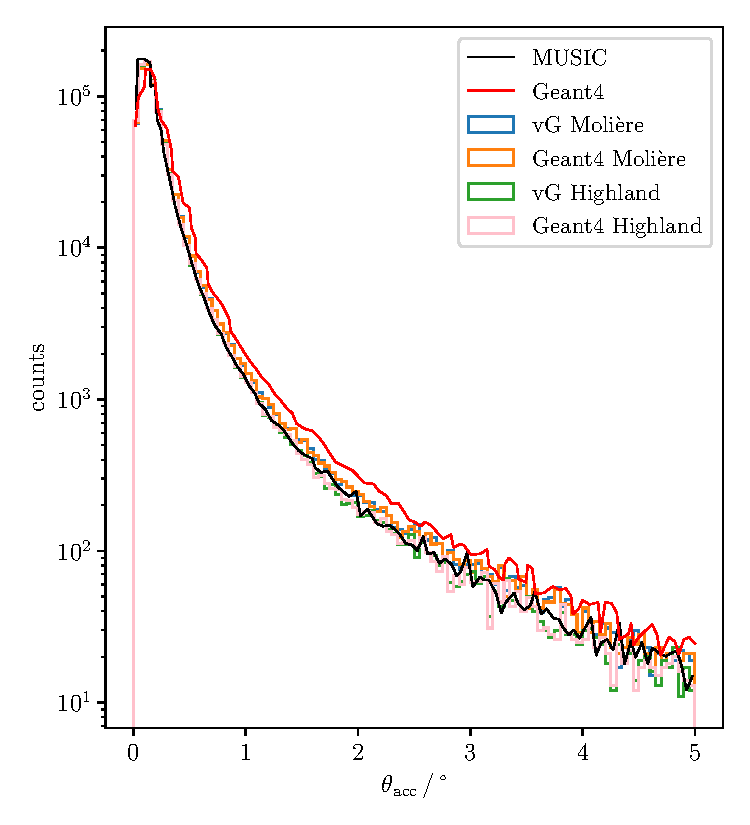
\includegraphics[width=0.48\textwidth]{../../deflection/plots/FINAL/2TeV_1e6events_accumulated_defl_only3km_5deg_paper.pdf}}
    \subcaptionbox{
        The lateral displacement $x$ in meter depends 
        on the scattering method. Molière scattering leads to larger distances.
        \label{fig:compare_MUSIC_dist}}
        {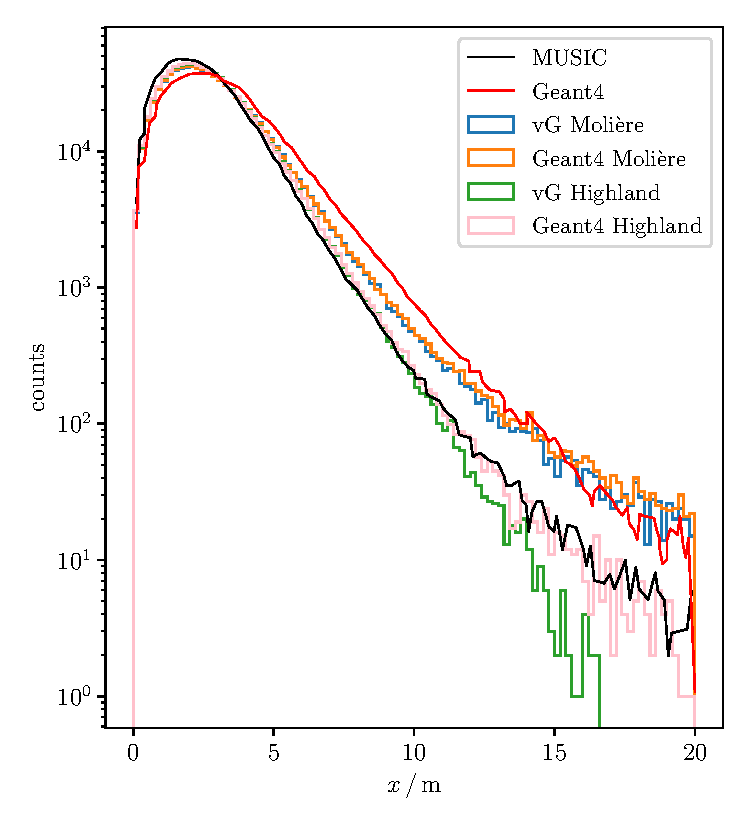
\includegraphics[width=0.48\textwidth]{../../deflection/plots/FINAL/2TeV_1e6events_distance_showeraxis_only3km_20m_paper.pdf}}
    \caption{A comparison of the results of MUSIC, GEANT4 and PROPOSAL is presented for $\num{1000000}$ negative charged muons propagated with 
    $E_{\text{i}} = \SI{2}{\tera\electronvolt}$ over a distance of 
    $\SI{3}{\kilo\meter}$ in water. A $\texttt{v\_cut} = 0.001$ is set. In PROPOSAL, 
    bremsstrahlung and photonuclear interaction are parametrized by 
    Van Ginneken (vG) and GEANT4 and both scattering methods are checked. Detailed information are given in 
    Table~\ref{tab:compare_MUSIC}. The results for MUSIC and GEANT4 are taken from 
    \cite{comparison_MUSIC_GEANT4_2009}.}
    \label{fig:compare_MUSIC}
\end{figure}



\begin{table}
    \small
    \centering
    \caption{The survival probability $p_{\text{s}}$ - otherwise the muon decays before, the mean survived muon 
    energy $\overline{E}_{\text{f}}$, the mean scattered angle $\overline{\theta}$ 
    and the mean displacement $\overline{x}$ are presented for all cases from 
    Figure~\ref{fig:compare_MUSIC}. For all means, the standard deviation is given.
    The largest deflection and displacement result in the tool GEANT4, which has the lowest mean survived energy. The lower the energy, the larger the deflection.}
    \begin{tabular}{l|cc|cccc}
        \toprule
        & & & \multicolumn{4}{c}{PROPOSAL} \\
        &  & & \multicolumn{2}{c}{Molière} & \multicolumn{2}{c}{Highland} \\
        & MUSIC & GEANT4 & vG & GEANT4 & vG & GEANT4 \\
        \midrule
        $p_{\text{s}}\,/\,\si{\percent}$ & 77.9 & 79.3 &  \multicolumn{4}{c}{77.9}\\
        $\overline{E}_{\text{f}}\,/\,\si{\giga\electronvolt}$ & 323 & 317 & \multicolumn{4}{c}{331$\pm$178} \\
        $\overline{\theta}\,/\,\si{\degree}$ & 0.22 & 0.27 & 0.24$\pm$0.45 & 0.24$\pm$0.45 & 0.22$\pm$0.35 & 0.22$\pm$0.35   \\
        $\overline{x}\,/\,\si{\meter}$ & 2.6 & 3.3 & 2.9$\pm$2.6 & 2.9$\pm$2.6 & 2.7$\pm$1.6 & 2.7$\pm$1.7  \\
     \bottomrule
    \end{tabular}
    \label{tab:compare_MUSIC}
\end{table}




For current analyses, it is important to study the impact of the muon 
deflection on the angular resolution to estimate an uncertainty on the reconstruction.
For this purpose, four different initial energies 
from $E_{\text{i}} = \SI{10}{\tera\electronvolt}$ to 
$E_{\text{i}} = \SI{10}{\peta\electronvolt}$ are used and the final 
energy is set to $E_{\text{f,\,min}} \geq \SI{10}{\giga\electronvolt}$ with 
$E_{\text{f,\,min}} < E_{\text{i}}$ for each simulation. To compare the results of 
a total of $\num{36}$ simulations, the median of the deflection distribution 
with a $\SI{95}{\percent}$ central interval is presented in 
Figure~\ref{fig:fit_median}.
The lower the final muon energy, the larger the accumulated deflection. 
For energies $E_{\text{f}} = \SI{1}{\peta\electronvolt}$, the median deflection 
is lower than $\SI{e-3}{\degree}$. For energies $E_{\text{f}} = \SI{10}{\giga\electronvolt}$, 
angles larger than $\SI{1}{\degree}$ are possible. For an energy range 
$E_{\text{f}} \approx \SI{500}{\giga\electronvolt} - \SI{1}{\tera\electronvolt}$, 
there is a small overlap of the deflection with the angular resolution of KM3NeT 
\cite{KM3NeT_Resolution2016}. The resolution of IceCube is a bit worse and 
therefore not affected \cite{IceCube_Resolution2021}. Since these simulations are done 
in ice, the same simulations are done in water. The deviations of the medians
are less than $\SI{1}{\percent}$ for all energies.

Furthermore, in Figure~\ref{fig:fit_median} there are only $12$ medians visible, 
instead of $36$ which is the total amount of all simulations. This result points 
out that the total deflection of a muon 
primarily depends on the final muon energy.
The initial muon energy is negligible. 
Hence, the reconstructed muon 
energy in a detector can be used to estimate a theoretical deflection. For this 
purpose, the following fit-function 
\begin{equation}
     f(x) = a \cdot x^3 + b \cdot x^2 + c \cdot x + d \,,
    \label{eqn:fit_median}
\end{equation}
can be applied with the parameters 
\begin{align}
    a =& +0.024 \pm 0.001\,,  & c =& +0.379 \pm 0.057\,,\\
    b =& -0.312 \pm 0.016\,,  & d =& -0.216 \pm 0.058\,,
\end{align}
in the logarithmic space via 
\begin{align}
    g(x) =& 10^{f(x)}\,, & x =& \log_{10}\left(\frac{E_{\text{f}}}{\si{\giga\electronvolt}}\right)\,.
\end{align}

\begin{figure}
    \centering 
    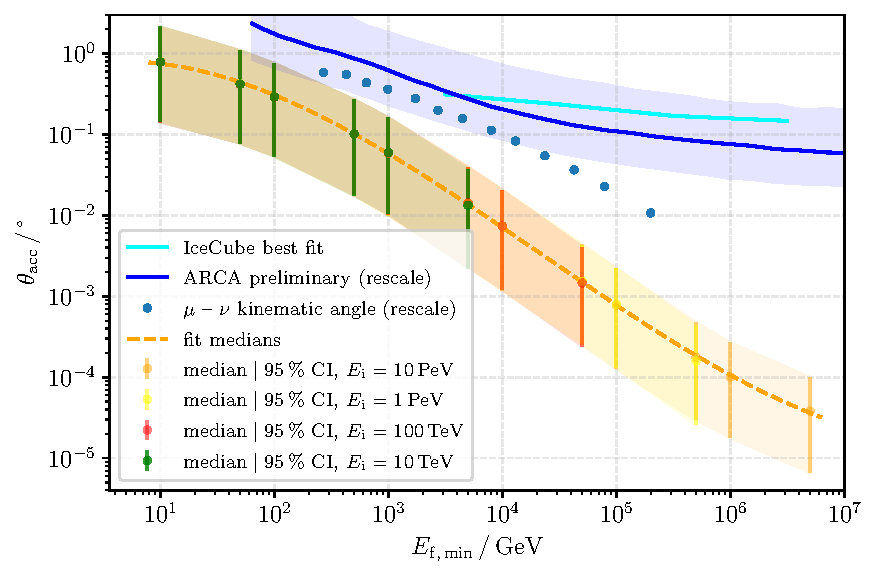
\includegraphics[width=0.96\textwidth]{../../deflection/plots/FINAL/fit_median_defl_cut_10percent_only_poly_new_resolution_rescale_no_icecube_paper_final.pdf}
    \caption{The median of the accumulated deflection $\theta_{\text{acc}}$ in degree 
    with a $\SI{95}{\percent}$ 
    central interval is shown for four different initial energies $E_{\text{i}}$. 
    Each data set includes more than $\num{50000}$ events with the requirement 
    that the true final particle energy $E_{\text{f}}$ is maximum 
    $\SI{10}{\percent}$ below the set final energy $E_{\text{f,\,min}}$,   
    $E_{\text{f}} > E_{\text{f,\,min}} \cdot 0.9$. The energy cuts are $\texttt{e\_cut} = \SI{500}{\mega\electronvolt}$ and $\texttt{v\_cut} = 0.05$ and 
    Molière scattering is chosen. Simulations are done in ice, the deviation 
    of the medians in a water based simulation are less than $\SI{1}{\percent}$.
    Since the medians overlap for different initial energies, there is no 
    strong impact of the initial energy on the median deflection. These 
    medians can be fit by a third degree polynomial in the log-space as 
    shown in Equation~\ref{eqn:fit_median}. For energies 
    $E_{\text{f}} \approx \SI{500}{\giga\electronvolt} - \SI{1}{\tera\electronvolt}$, there is a minimal influence of deflection on the angular resolution of 
    KM3NeT \cite{KM3NeT_Resolution2016}. The resolution of IceCube is not 
    impacted \cite{IceCube_Resolution2021}.}
    \label{fig:fit_median}
\end{figure}

\textcolor{red}{$E_{\text{f}}$ und $E_{\text{f,\,min}}$ eindeutig und konsistent verwenden!}

\textcolor{red}{Fig3 beinhaltet noch keine neutrino-energy korrektur! der neueste plot ist in figures/fit\_median\_defl\_cut\_10percent\_only\_poly\_resolution\_rescale\_no\_icecube.pdf}

% \textcolor{red}{umrechnung der neutrinoenergie in myonenergie: northerntrack sample verwenden, dort einfach reinschauen mit welchen energien werden die neutrinos injeziert, welche muon energien kommen dabei raus -- dieses sample wird verwendet, da es für point source analysis relevant ist -- die gewichtung des spektrums muss berücksichtigt werden -- dort nachschauen, welches spektrum verwendet wird für astro}

\section{Conclusion}
\section{Acknowledgement}

%% The Appendices part is started with the command \appendix;
%% appendix sections are then done as normal sections
%% \appendix

%% \section{}
%% \label{}

%% If you have bibdatabase file and want bibtex to generate the
%% bibitems, please use
%%
\bibliographystyle{elsarticle-num} 
\bibliography{lit.bib}


%% else use the following coding to input the bibitems directly in the
%% TeX file.

% \begin{thebibliography}{00}

%% \bibitem{label}
%% Text of bibliographic item

% \bibitem{bibtest}Peter Pan, Uni Dortmund
% \bibitem{b2}Pascal, 2. Test

% \end{thebibliography}
\end{document}
\endinput
%%
%% End of file `elsarticle-template-num.tex'.
